% \documentclass[11pt,mathserif]{beamer}
\documentclass[11pt]{beamer}

\usepackage[english]{babel}
\usepackage{pgf}
\usepackage{amsmath,amssymb,wasysym}
\usepackage[latin1]{inputenc}
\usepackage{multirow}
\usepackage{graphicx}
\usepackage{ulem}
\usepackage{color}
\usepackage{comment}
\usepackage{hyperref}
\usepackage{listings}
\usepackage{tabularx}
\usepackage{verbatim}

%\lstnewenvironment{code}{\lstset{language=C,basicstyle=\scriptsize\ttfamily}}{}

\definecolor{dred}{RGB}{200,0,0}
\definecolor{dgreen}{RGB}{0,150,0}

\mode<presentation>
{
  \useinnertheme{rectangles}
  \useoutertheme{split}
  \setbeamerfont{block title}{size={}}
  \usefonttheme{structurebold}
  \usecolortheme{Intel}
  \setbeamercovered{transparent}
}

\pgfdeclareimage[width=3.0cm]{intel-logo}{intel2}
\titlegraphic{
  \pgfuseimage{intel-logo}
}

\title[PGAS Tutorial]{Overview of HW/SW landscape for PGAS}
\author[Jeff Hammond]{Jeff Hammond}
\institute[Intel Labs]{Extreme Scalability Group \& Parallel Computing Lab\\ Intel Corporation (Portland, OR)}
\date[]{26 September 2014}

\begin{document}

\frame{\titlepage}

\begin{frame}{}
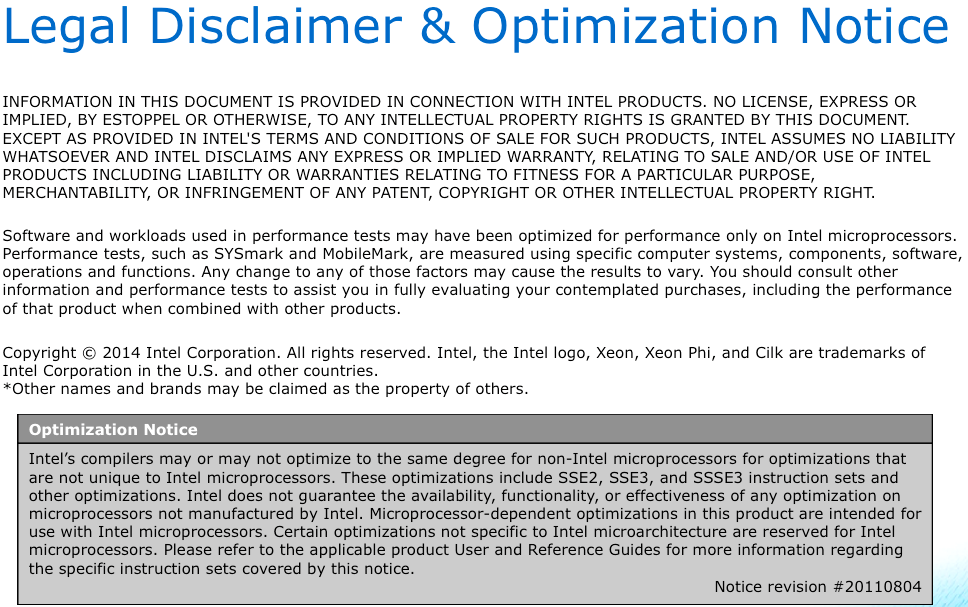
\includegraphics[scale=0.33,angle=0]{intel-legal} \
\end{frame}

\begin{frame}{} \LARGE
  \begin{center}
      \textbf{From Intel Xeon Phi to PGAS\ldots}
  \end{center}
\end{frame}

\begin{frame}{Motivation} \large
    \begin{itemize}
        \item Generation 1 (Knights Corner) Xeon Phi is coprocessor.
        \item Native supported, but offload prevalent.  PGAS not about offload.
        \item PCI bus is a huge impediment to performance and programmability.
        \item Generation 2 (Knights Landing) socketized, packaged with Aries network.
        \item The future is many-core with a tightly integrated network.
        \item The best proxy for a KNL node is a KNC card.
    \end{itemize}
    See for details: \\
    \url{http://tinyurl.com/ltjmdvj} \url{http://tinyurl.com/myxzr3j}
    % http://goparallel.sourceforge.net/nersc-supercomputer-first-use-intels-next-gen-knights-landing/
    % http://newsroom.intel.com/community/intel\_newsroom/blog/2014/06/23/intel-re-architects-the-fundamental-building-block-for-high-performance-computing
\end{frame}

\begin{frame}{} \LARGE
  \begin{center}
      \textbf{MPI+X}
  \end{center}
\end{frame}

\begin{frame}[fragile]{The future is MPI+X (supposedly)} \large
\begin{itemize}
	\item MPI+OpenMP is too often fork-join.
	\item Pthreads scare people; can't be used from Fortran (easily).
	\item Intel$^\circledR$ has Cilk$^\circledR$ and TBB.
	\item OpenCL is not a good model for application programmers
          and has no magic for portable performance (since such magic does not exist).
    \item Do C++11 thread/async features make sense in HPC?
\end{itemize}
Never confuse portability with portable performance!
\end{frame}

\begin{frame}{Using MPI+OpenMP effectively} \large 
\begin{itemize}
	\item Private data should behave like MPI but with load-store for comm.
	\item Shared data leads to cache reuse but also false sharing.
	\item NUMA is going to eat you alive.  Blue Gene is a rare exception.
	\item OpenMP offers little to no solution for NUMA.
	\item If you do everything else right, Amdahl is going to get you.
\end{itemize}
Intranode Amdahl and NUMA are giving OpenMP a bad name;
fully rewritten hybrid codes that exploit affinity behave very different
from MPI codes evolved into MPI+OpenMP codes.
\end{frame}

\begin{frame}{Fork-Join vs. Parallel-Serialize}
  \begin{center}
    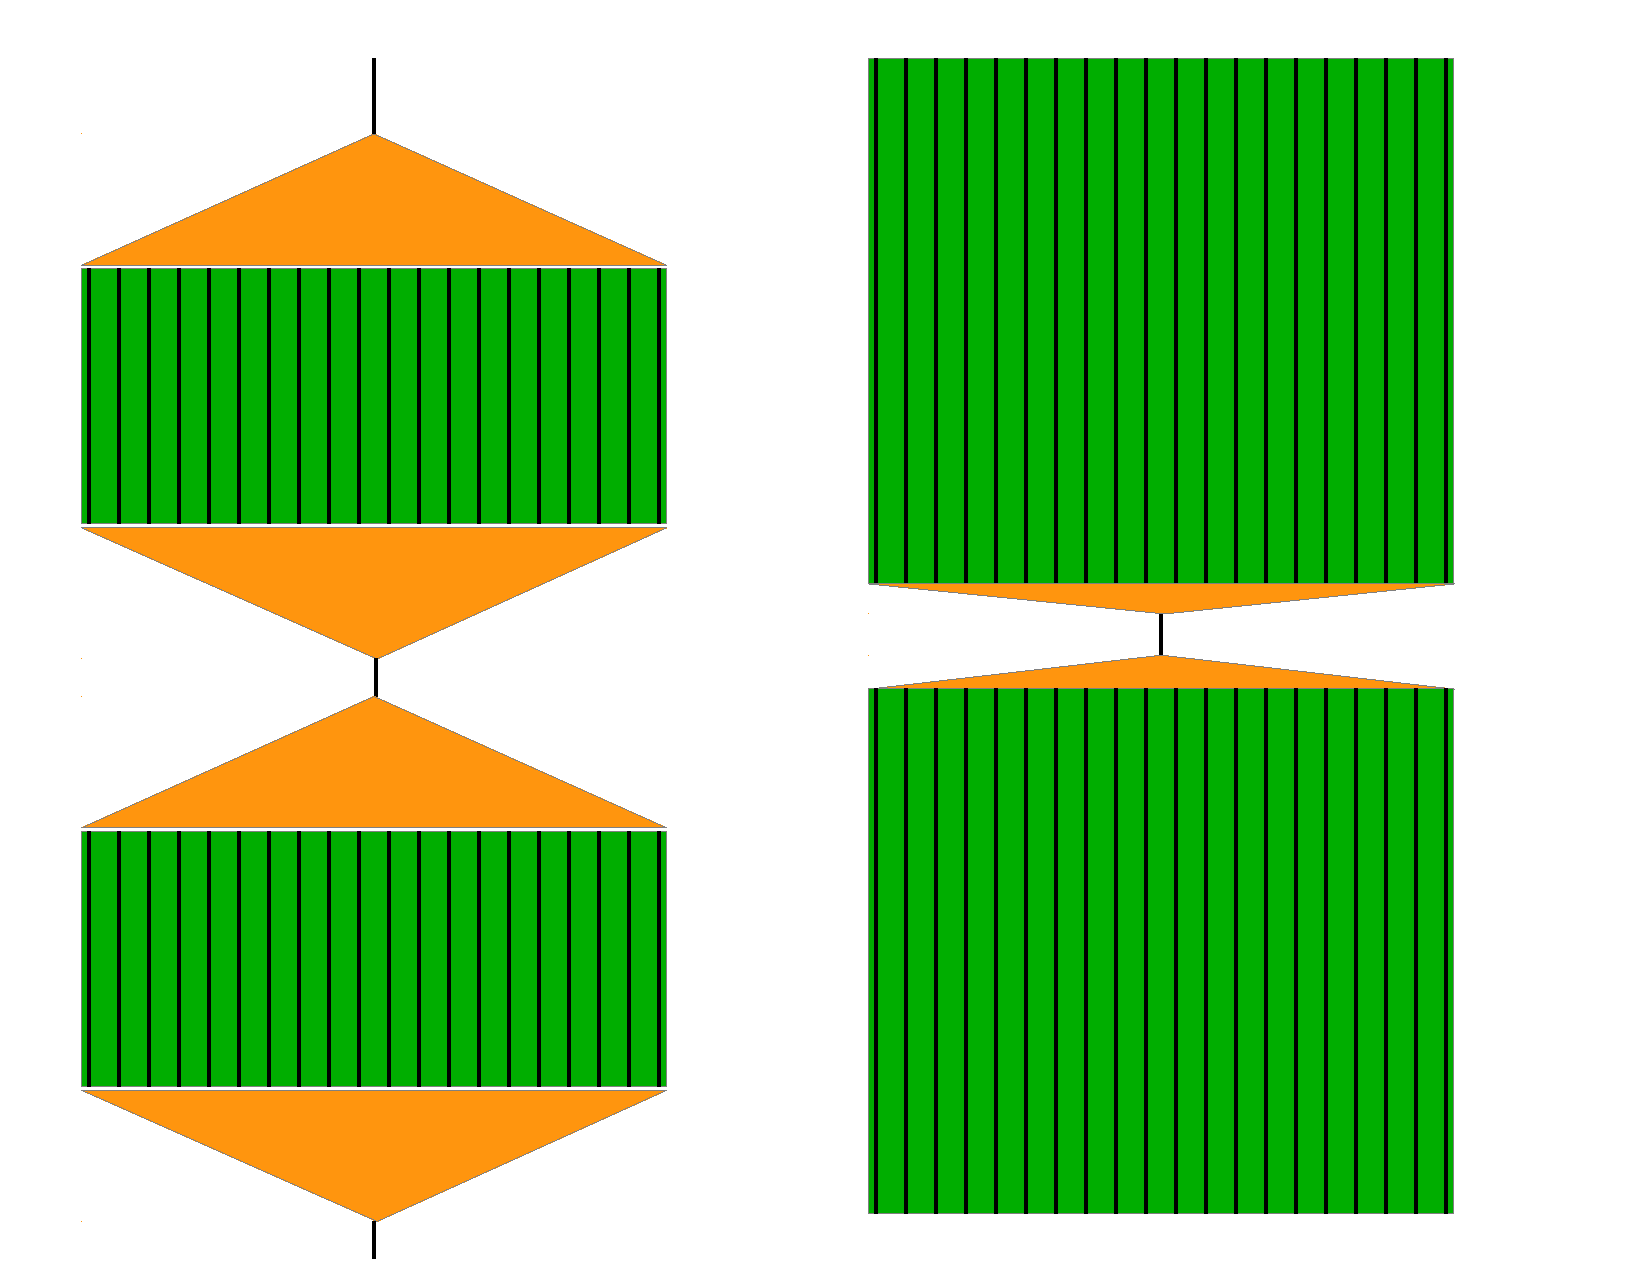
\includegraphics[scale=0.3,angle=0]{ForkJoin.pdf}
  \end{center}
\end{frame}

\begin{frame}{Fork-Join vs. Parallel-Serialize}
  \begin{columns}[T]
    \begin{column}{0.5 \linewidth}
      \begin{tt}
       \color{black}
       \#pragma omp parallel       \\
       \{ \\
       \color{green}
       /* thread-safe */      \\
       \vskip1ex
       \color{black}
       \#pragma omp single         \\
       \color{red}
       /* thread-unsafe */    \\
       \vskip1ex
       \color{black}
       \#pragma omp parallel for   \\
       \color{green}
       /* threaded loops */ \\
       \vskip1ex
       \color{black}
       \#pragma omp sections       \\
       {\color{green}
       /* threaded work */}  \\
       \}     \\
      \end{tt}
    \end{column}
    \begin{column}{0.5 \linewidth}
      \begin{tt}
       {\color{red} /* thread-unsafe */ }  \\
       \vskip1ex
       \color{black}
       \#pragma omp parallel for \\
       \{ \\
       {\color{green} /* threaded loops */} \\
       \} \\
       \vskip1ex
       {\color{red} /* thread-unsafe */ }  \\
       \vskip1ex
       \color{black}
       \#pragma omp parallel for \\
       \{ \\
       {\color{green} /* threaded loops */ } \\
       \} \\
       \vskip1ex
       \color{red}
       /* thread-unsafe work */  \\
      \end{tt}
    \end{column}
  \end{columns}
\end{frame}

\begin{frame}{MPI funneling bad} \Large
    \begin{itemize}
        \item Transition to parallelism for increased performance
              within processors and networks.
        \item Must exploit network parallelism to max out hardware
              for small messages.
        \item More overlap opportunity and latency-hiding with 
              greater communication concurrency.
        \item Blue Gene/Q good example of needing+supporting network parallelism.
    \end{itemize}
\end{frame}

\begin{frame}{} \LARGE
  \begin{center}
      \textbf{MPI$\otimes$X}
  \end{center}
\end{frame}

\begin{frame}{MPI$\otimes$X} \large 
\begin{itemize}
    \item Threads are independent, long-lived tasks in a shared address space.
    \item Threads all access MPI like they own it.
    \item \texttt{MPI\_THREAD\_MULTIPLE} is non-trivial overhead.
    \item Be sure you have a communicator per thread with collectives\ldots
    \item If your low-level network stack is not thread-safe\ldots
    \item God help you if you want to mix more than one threading model!$^{1}$
    \item Jim Dinan will bring about \texttt{MPI\_WORLD\_PEACE} with endpoints :-)
\end{itemize}
\vskip1ex
{\small $^{1}$ See \url{https://www.ieeetcsc.org/activities/blog/challenges_for_interoperability_of_runtime_systems_in_scientific_applications} }
\end{frame}

\begin{frame}{} \LARGE
  \begin{center}
      \textbf{MPI+MPI}
  \end{center}
\end{frame}

\begin{frame}{Best of all worlds?}
    MPI-3 between nodes; MPI-Shm within the node\ldots
    \begin{itemize}
        \item Private by default; shared by request.  Safe.
        \item Memory affinity to each core; NUMA issues should be rare.
        \item No fork-join - end-to-end parallel execution, 
              just a question of replicated or distributed (GA-like).
        \item No need to reimplement \textit{any} collectives.
        \item Easily supports both task- and data-parallelism.
        \item Hierarchy via MPI communicators.
        \item One runtime to rule them all.  No interop BS.
        \item \texttt{MPI\_THREAD\_SINGLE} sufficient.
    \end{itemize}
\end{frame}

\begin{frame}{Why not MPI+MPI?} \Large
    \begin{itemize}
        \item MPI shm allocation collective.
        \item MPI shm allocator not \texttt{malloc}.
        \item No cure for data races.
        \item Data races not cured.
        \item cured. races not Data
        \item All the intranode libraries use threads!!!
    \end{itemize}
\end{frame}

\begin{frame}{} \LARGE
  \begin{center}
      \textbf{PGAS}
  \end{center}
\end{frame}

\begin{frame}{PGAS - Pro} \Large
    \begin{itemize}
        \item Similar to MPI$\otimes$X and MPI+MPI.
        \item No fork.  No join.
        \item Always had the NUMA situation in-order.
        \item Not shared memory.  False sharing less likely.
    \end{itemize}
\end{frame}

\begin{frame}{PGAS - Con} \Large
    \begin{itemize}
        \item Looks flat.  Multi-node multi-core is not.
        \item Implicit communication is evil (duck!).
        \item Silent on SIMD issues for wide vector FPU.
        \item Implementation situation\ldots
        \item Wider portability issues\ldots
        \item RDMA through PCI is extra hops.
    \end{itemize}
\end{frame}

\begin{frame}{} \LARGE
  \begin{center}
      \textbf{PGAS Hybrids}
  \end{center}
\end{frame}

\begin{frame}{PGAS+X} \Large
    \begin{itemize}
        \item Eliminate the flatness - use X within node.
        \item X might help with SIMD, other fine-grain issues.
        \item Runtime and implementation difficulties?
        \item Less of an issue if/when PGAS uses threads within the node.
    \end{itemize}
\end{frame}

\begin{frame}{MPI+PGAS} \Large
    \begin{itemize}
        \item MPI-1 very successful for distributed memory;
              PGAS obviously going to work well in shared-memory.
        \item PGAS is vastly superior to non-expert OpenMP w.r.t. fork-join.
        \item MPI-PGAS rivalry created unfortunate sociological barrier to this model.
        \item Since MPI-3 RMA is PGAS, most likely instantiation is MPI+MPI :-)
    \end{itemize}
\end{frame}

\begin{frame}{} \LARGE
  \begin{center}
      \textbf{The Rest of the Day}
  \end{center}
\end{frame}

\begin{frame}{} \Large
    \begin{itemize}
        \item Bottom-up: SFI$\rightarrow$MPI-3$\rightarrow$UPC
        \item MVAPICH2-X brings MPI-3 and PGAS together.
        \item OSHMPI (OpenSHMEM over MPI-3) can be used on MIC.
        \item Tutorial hardware generously provided by Sameer.
        \item Performance experiments discouraged for multiple reasons.
        \item Hands-on starts out structure\ldots
    \end{itemize}
\end{frame}

\end{document}
